\section{\ApproachName}
% 为了能够提取可视化算法中的信息,\ApproachName 采用了原始数据和可视化算法作为输入,以提取的编码信息作为输出。
% 这里,原始数据指的是输入的图数据,我们采用了常用的nodes-links格式的json格式作为图数据的标准格式,其他格式的数据可以通过简单的转化变成json格式;
% 可视化算法指的是一种将数据本身映射到屏幕上的图形的算法,具体的,在前端编程环境下,指的是将原始数据映射为svg树的过程。

% 我们将编码信息进行了定义,其包含四部分:数据元、数据属性、图形、通道。
% 其中数据元指的是一个节点或一个链接,数据属性指的是数据元上的属性,图形指的是一个svg元素,而通道则是指该元素可以用来编码的属性。
% 举例而言,。。。
% 于是,一条编码方案就可以被描述为数据元的某个属性映射到图形的某个通道。
% 算法的目标可以被总结为:
% 1. 为节点和链接找到

% % 我们提出了xxx,通过抽取信息并填充模板的方式来描述节点链接图,它大概分为三个步骤~\REf{}:1. xxx; xxx
% We introduce \ApproachName, which describes node-link diagrams by extracting information and filling templates.
None of these approaches is tailored for generating descriptions for node-link diagrams. 
We propose an approach named \ApproachName~to generate descriptions for node-link diagrams automatically.
It utilizes three information extraction pipelines to detect crucial information from the source code and the underlying graph and generates template-based descriptions.
The pipeline of \ApproachName~consists of three steps (Figure~\ref{fig:workflow}), which interprets:
\textbf{1) linking conditions} to describe how nodes relationships are constructed by finding, filtering, and sorting conditions;
\textbf{2) visual encodings} by extracting visual mappings among data entities, attributes, visual elements, and visual channels; and
\textbf{3) layout intention} by identifying different kinds of layouts and their affecting factors.

We implement an interactive interface based on \ApproachName, in which creators can input the source code and data to generate node-link diagrams and descriptions.
We augment the generated descriptions by highlighting interactions to enhance understanding.
When audiences hover on sentences of descriptions, relevant parts of the diagram are highlighted.

\begin{figure}
    \centering
    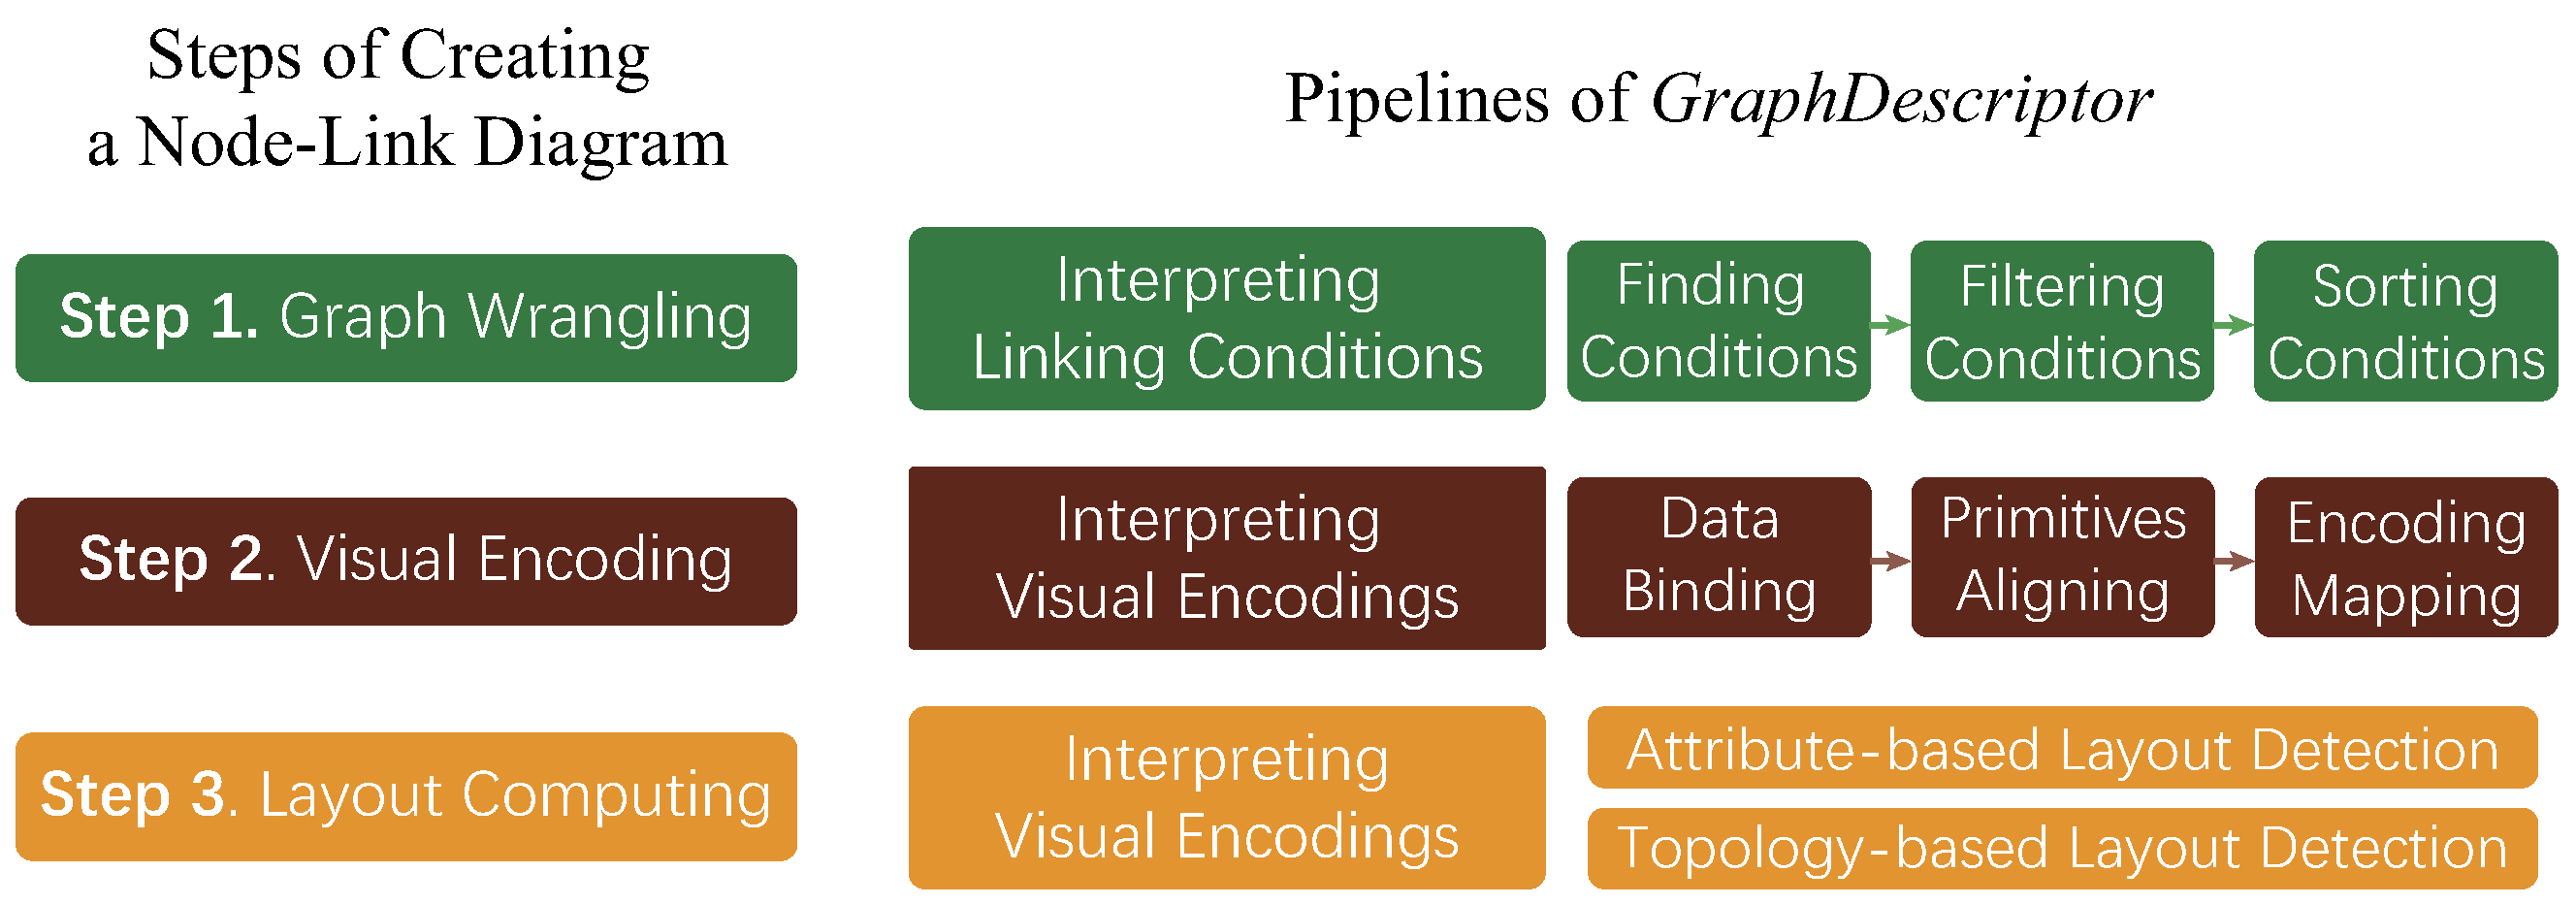
\includegraphics[width=1\columnwidth]{figures/workflow.eps}
    \caption{The pipeline of \textit{\ApproachName} follows the three-step creation process of node-link diagrams to interpret linking conditions, visual encodings, and layout intention.}
    \label{fig:workflow}
\end{figure}


\subsection{Interpreting Linking Conditions}
% 从表格型数据创建图数据时,最重要的就是建立节点之间的关系。
% 观众从节点链接图中所能获知的信息仅仅是某两个节点之间存在联系,但却不了解联系的内在含义。
% 一些论文已经对可能建立链接的情况进行了定义,
Several techniques~\cite{DBLP:journals/ivs/LiuNS14, DBLP:journals/ivs/HeerP14, DBLP:journals/tvcg/SrinivasanPEB18} of graph wrangling identify link construction as the crucial process and propose several linking conditions.
Thus our technique describes linking conditions to interpret the graph wrangling step.
Ploceus~\cite{DBLP:journals/ivs/LiuNS14} and Orion~\cite{DBLP:journals/ivs/HeerP14} infer potential linking conditions by constructing a linking graph and searching valid linking paths. They construct links among multiple data tables by analyzing primary and foreign keys.
Graphiti
Graphiti~\cite{DBLP:journals/tvcg/SrinivasanPEB18} identifies potential linking conditions of a homogeneous graph by comparing different attributes.
% 如果多个表合并成一个表,前两者总结的条件可以被Graphiti提出的规则所覆盖
Because multiple tables can be merged into one data table with primary and foreign keys, Graphiti can cover the linking conditions by identifying Ploceus's and Orion's rules.
Those works infer the potential linking conditions when only a few links are constructed;
% 我们尝试从它们的反方向进行思考,也就是,当我们获取到了所有的链接的时候,推测这些链接是如何被构建的
our method, on the other hand, works in the opposite direction from already constructed links.

\textbf{Finding Conditions}. We first construct conditions between all pairs of nodes. The conditions summarized by Graphiti can be organized into four categories:
\begin{compactenum}[\textbf{C}1]
    % 两个节点的某个属性值相同
    \item Values of an attribute of two nodes are the same, e.g., linking two movies published in the same year.
    % 两个节点的某个属性拥有超过一个共同的值
    \item Two nodes have at least one common value of a list attribute, e.g., linking two movies with one or more of the same actors.
    % 两个节点的某个属性值非常接近
    \item Values of an attribute of the two nodes are significantly close, where \textit{significance} is defined by the normalized difference.
    \item Values of an attribute of two nodes are in the same bin, where the bins are separated by quartiles.
\end{compactenum}

% 为了能够将这些condition填充到文本模板中,我们对condition的输出进行了formalize
We formalize the conditions with three aspects to facilitate comparison, sorting and filtering.
One condition can be defined as:
\begin{equation}
    linking\text{ }condition := ( type, attribute, value )
\end{equation}
where $type$ is the condition type, $attribute$ is the name of the attribute, $value$ is the value of the attribute when the condition holds.

\textbf{Filtering Conditions}.
We first detect linking conditions held on node pairs without any connections.
These conditions are regarded as false condition because no links exist, and should be filtered out.
Only conditions whose occurrences are no less than the number of links are selected from the rest conditions (Algorithm~\ref{alg:conditions}).

\textbf{Sorting Conditions}.
% After that, conditions are sorted by their \textit{degrees} and the highest-ranked condition will be regarded as the most possible condition.
% Degrees of conditions can be compared by their implication relations.
After that, conditions are sorted by their degrees through the comparison of their implication relations, the highest-ranked condition is regarded as the most likely condition.
For example, the condition $(type=C2, attribute=actors, value=[Alice, Bob])$ is implied by $(type=C2, attribute=actors, value=[Alice])$ and $(type=C2, attribute=actors, value=arbitrary\text{ }value)$, where $(value=arbitrary\text{ }value)$ means the condition does not assume the $actors$ attribute should equal to a certain value.
Its has a higher degree than the others, and is thus ranked higher.

We textualize the linking condition of the graph by filling templates. 
Four templates correspond to four conditions according to the $type$:
\begin{compactenum}[\textbf{T}1]
    \item \textit{``Two nodes are connected if the values of the attribute $@attribute$ are the same\$\{ ($@value$)?\}''}.
    \item \textit{``Two nodes are connected if the values of the attribute $@attribute$ have common values\$\{ ($@value$)?\}}''.
    \item \textit{``Two nodes are connected if the values of the attribute $@attribute$ are close (with a difference less than $@value$)''}.
    \item \textit{``Two nodes are connected if the values of the attribute $@attribute$ are within the same \$\{$@value$ ?\}bin''}.
\end{compactenum}
Here \$\{?\} means an included part that can be omitted and $@$ represents a placeholder.
For example, two movies sharing the same actors Alice and Bob are connected under the Condition \textbf{C2}, which could be represented as: $(type=C2, attribute=actors, value=[Alice, Bob])$. 
Its corresponding description is: \textit{``Two nodes are connected if the values of the attribute actors have common values ([Alice, Bob])''}. 
For the condition $(type=C2, attribute=actors, value=arbitrary\text{ }value)$, contents in its parentheses are omitted.

\begin{algorithm}[!t]
    \renewcommand\arraystretch{1.2}
    \caption{ Filtering Conditions }
    \label{alg:conditions}
    \begin{algorithmic}[1]
        \Require
            $G=(V=\{v_1, v_2, ..., v_n\}, E=\{e_1, e_2, ..., e_n\})$: a graph;
        \Ensure
            $C$: the potential condition set
        \State Init conditions $C=\varnothing$, false conditions $FC=\varnothing$
        \For {each node pair $(v_i, v_j)$}
            \If {$(v_i, v_j)$ is not a link}
                \State $C_{ij} \gets$ all conditions that can link $(v_i, v_j)$
                \State merge $FC$ with $C_{ij}$
            \EndIf
        \EndFor
        \For {each link $e_k=(v_i, v_j)$}
            \State $C_{ij} \gets$ all conditions that can construct link $e_i$
            \For {each condition $c$ in $C_{ij}$}
                \If {$c$ in $FC$}
                    \State remove $c$ from $C_{ij}$
                \EndIf
            \EndFor
            \State merge $C$ with $C_{ij}$
        \EndFor
        \For {each condition $c$ in the condition set $C$}
            \If {the frequency of $c$ is less than $|E|$}
                \State remove $c$ from $C$
            \EndIf
        \EndFor
        \State \Return $C$
    \end{algorithmic}
\end{algorithm}


\subsection{Interpreting Visual Encodings}\label{sec:visualencodings}
\subsubsection{Background}
% 为了在节点链接图中展示节点、链接的属性,常常将这些属性编码为节点/链接的视觉通道。
Creators often encode attributes of nodes and links by visual channels to reveal attribute-based patterns.
Nodes and links contained in the underlying graph are denoted as \textit{data entities} and each data entity consists of several \textit{attributes}.
For the node-link diagram example in Figure~\ref{fig:VisualEncodings}, a node contains a categorical attribute (\textit{x}) and a numerical list attribute (\textit{y}), We encode the list attribute \textit{y} with the height of two rectangles.
Then we encode the attribute \textit{x} with the two rectangles' fill color and the background rectangle's stroke color.

% 我们的方法处理的对象是基于SVG的。
\ApproachName~seeks to extract visual encodings from node-link diagrams in the SVG format, which is widely used in the visualization area.
Visualization creators can write programs with the W3C DOM API to construct visualizations within SVG.
A SVG includes a root element \texttt{<svg>} and allows hierarchical grouping of subelements with group elements \texttt{<g>}.
Marks onscreen are generated by graphical elements such as \texttt{<rect>}, \texttt{<circle>}, and \texttt{<ellipse>}.
We call these graphical elements \textit{visual elements}.
Their style attributes such as \texttt{cx}, \texttt{cy}, \texttt{width}, and \texttt{height} are denoted as \textit{visual channels}.
Each kind of visual elements has both unique channels (e.g., \texttt{width} and \texttt{height} are only owned by \texttt{<rect>}) and universal channels (e.g., \texttt{fill}, \texttt{stroke-width}).

\begin{figure}[ht]
    \centering
    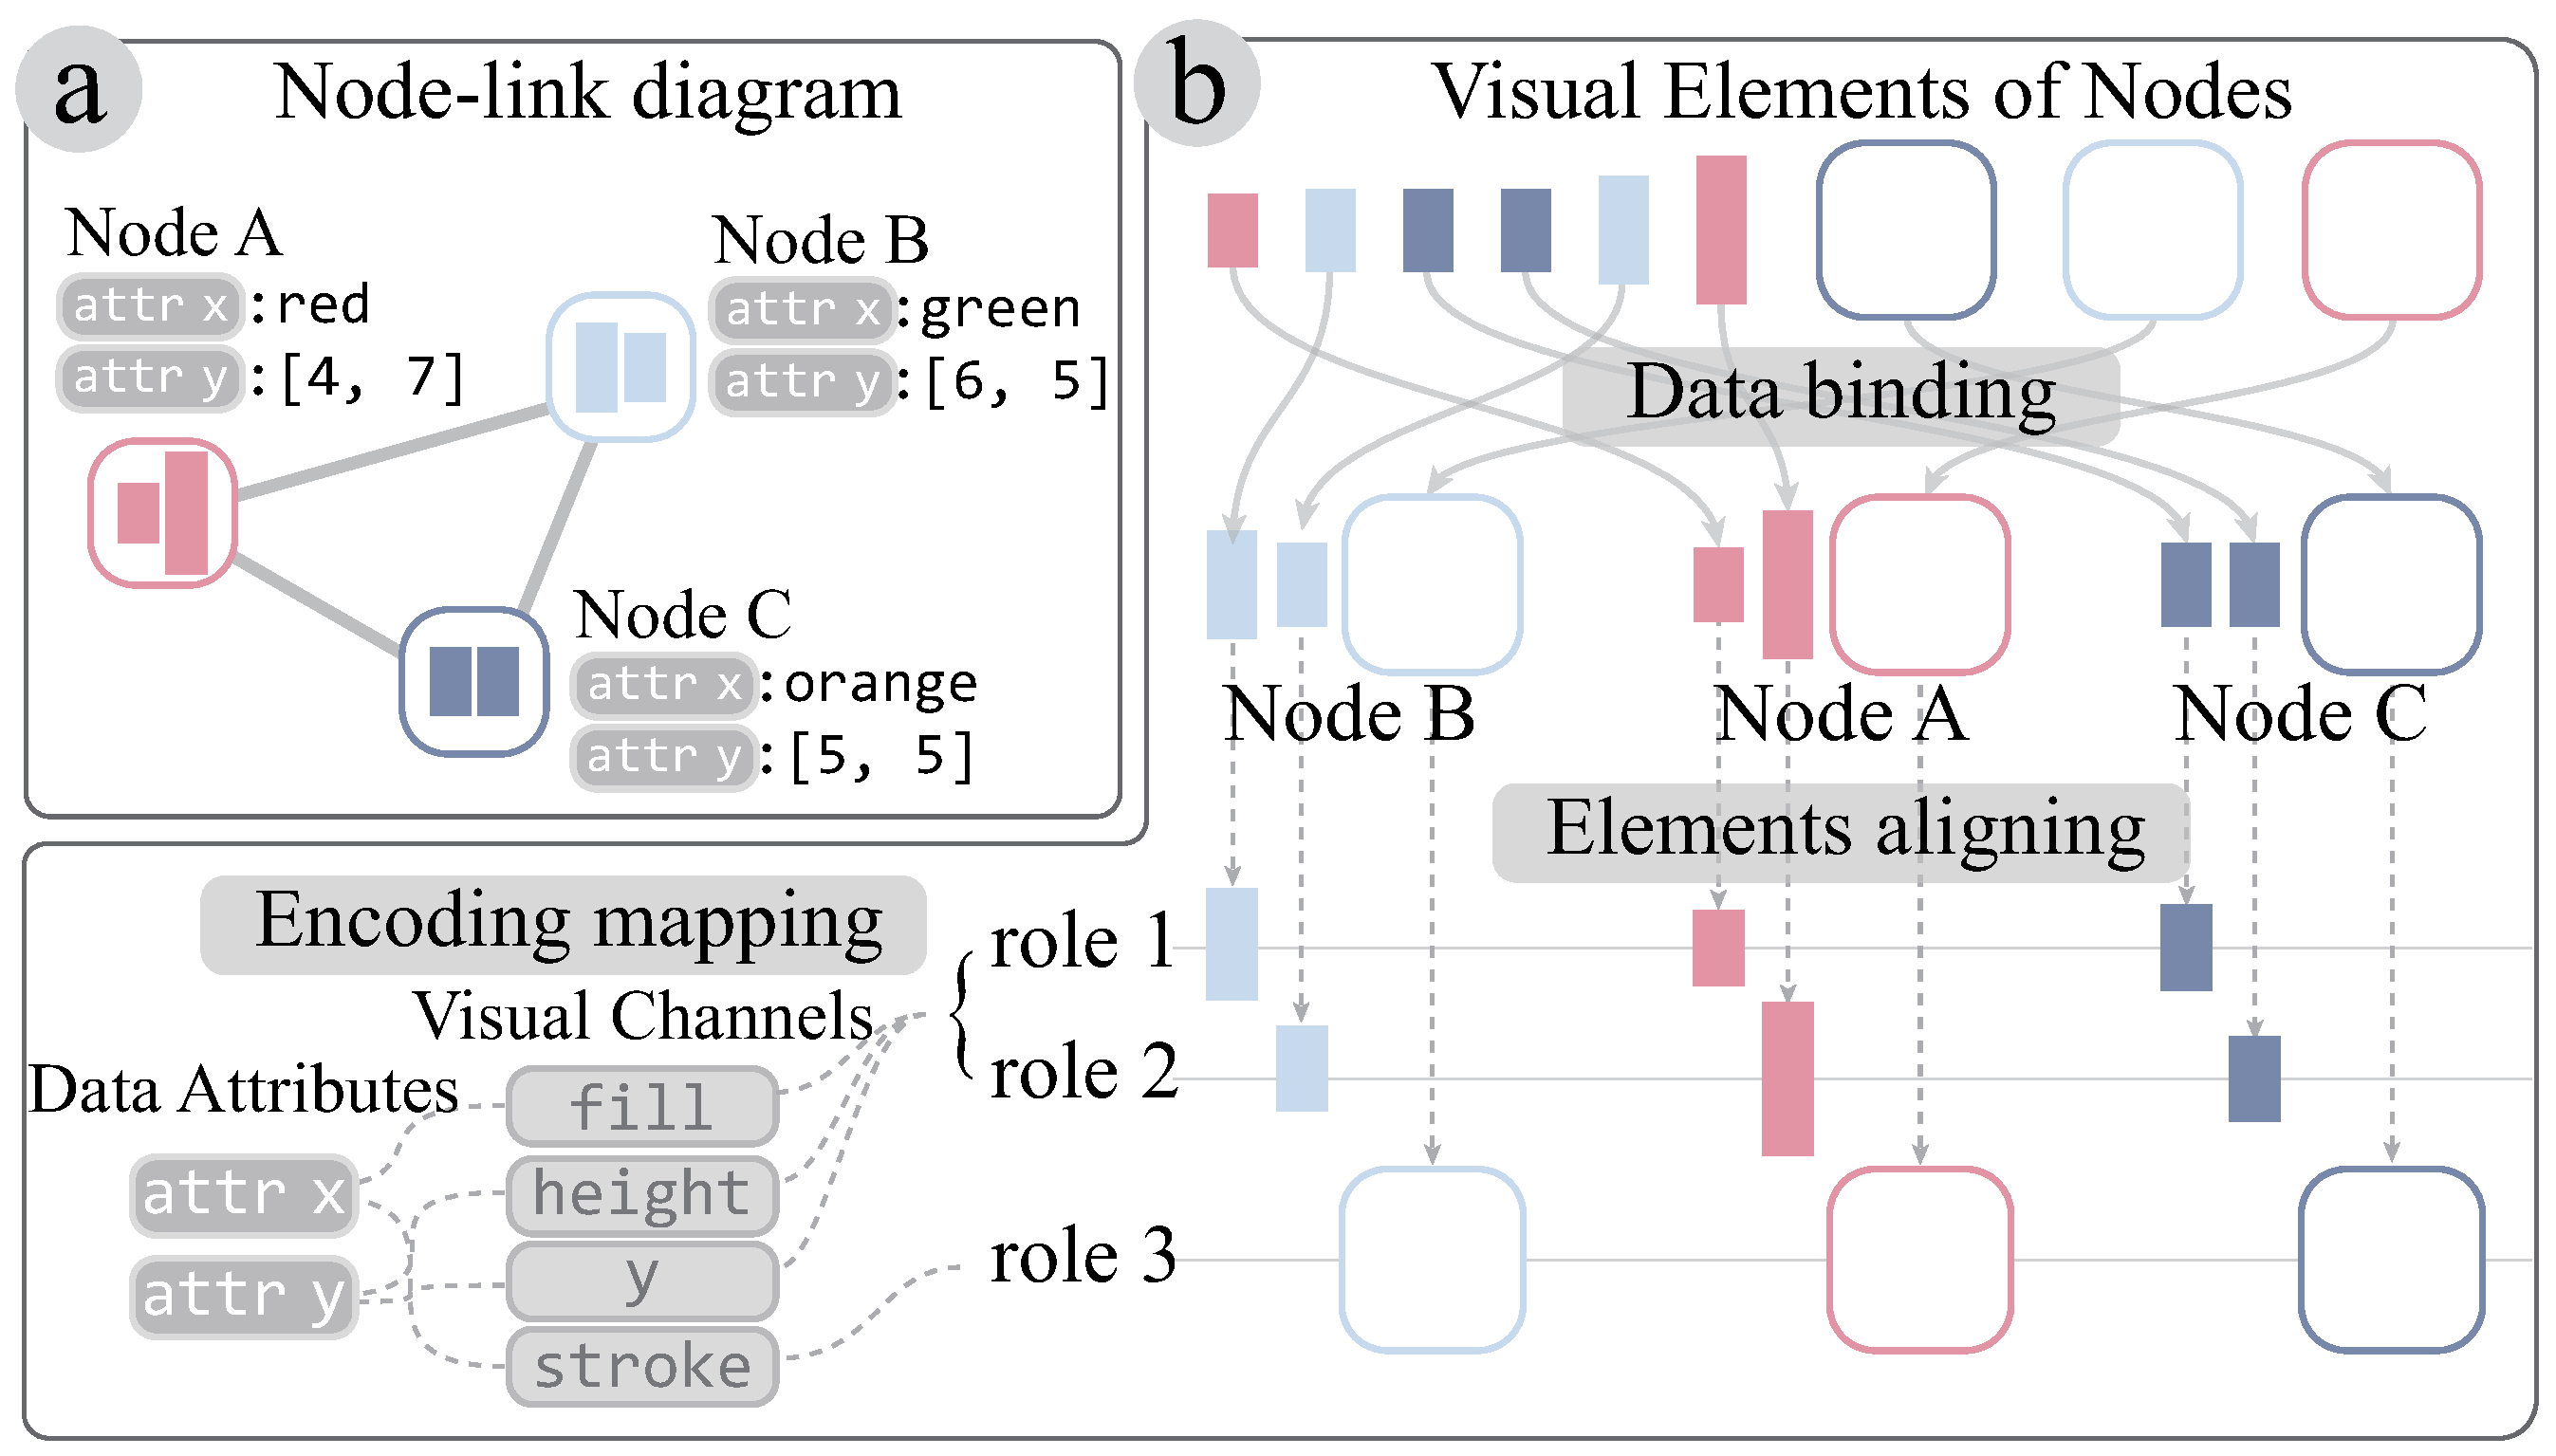
\includegraphics[width=1\columnwidth]{figures/VisualEncodings.eps}
    \caption{How \ApproachName~extracts visual encodings from a node-link diagram in the SVG format. A node-link diagram consists of three nodes and three links (upper left corner). Node elements are extracted and the \textbf {data binding} step maps them into different node entities. Then elements having the same role across different node entities are aligned into the same role class in the \textbf{elements aligning} step. Mappings among roles, visual channels, and attributes are detected by the \textbf{encoding mapping} step.}
    \label{fig:VisualEncodings}
\end{figure}

% 我们的工作通过分析源代码,从中提取数据实体()是如何被编码为视觉通道的()
We formulate the problem of describing visual encodings in node-link diagrams by three questions:
\begin{compactenum}[\textbf{Q}1]
    \item \textit{What elements does a node/link consist of in the diagram?} 
    For example, in Figure~\ref{fig:VisualEncodings}, a node is composed of three rectangles. \label{qstn:composition}
    
    \item \textit{What attributes do elements and their visual channels encode?} 
    For example, in Figure~\ref{fig:VisualEncodings}, the left rectangle's height in Node A encodes the first item of the attribute $y$. 
    % When the shape (\texttt{tagName}) of an element encodes some attribute, we should classify and discuss when elements are visualized as different shapes. 
    Attributes may be visualized in different ways according to the shape of the elements, such as the width and height of the \texttt{<rect>} and the radius of the \texttt{<circle>}.\label{qstn:encodings}
    % For example, when the node is encoded into a \texttt{<circle>}, the radius encodes its degree, and when the node is encoded into a \texttt{<rect>}, the width and the height encode its degree. 
    
    \item \textit{Is there a certain type of correlation (positive, negative, or categorical) between attributes and visual channels?}
    For example, the greater the degree of the node, the greater the radius of the circle.\label{qstn:correlation}
\end{compactenum}
Thus, it is necessary to extract mappings between \textbf{\textit{data entities}} and \textbf{\textit{visual elements}} and making correlations between \textbf{\textit{attributes}} and \textbf{\textit{visual channels}} to formulate the encoding scheme.

We define the encoding scheme as:
\begin{equation}
encoding := (entity, attribute, element, channel).
\end{equation}
Our target is to identify the entire set of encodings (Figure~\ref{fig:ElementAligning} (a)).

\begin{figure}[ht]
    \centering
    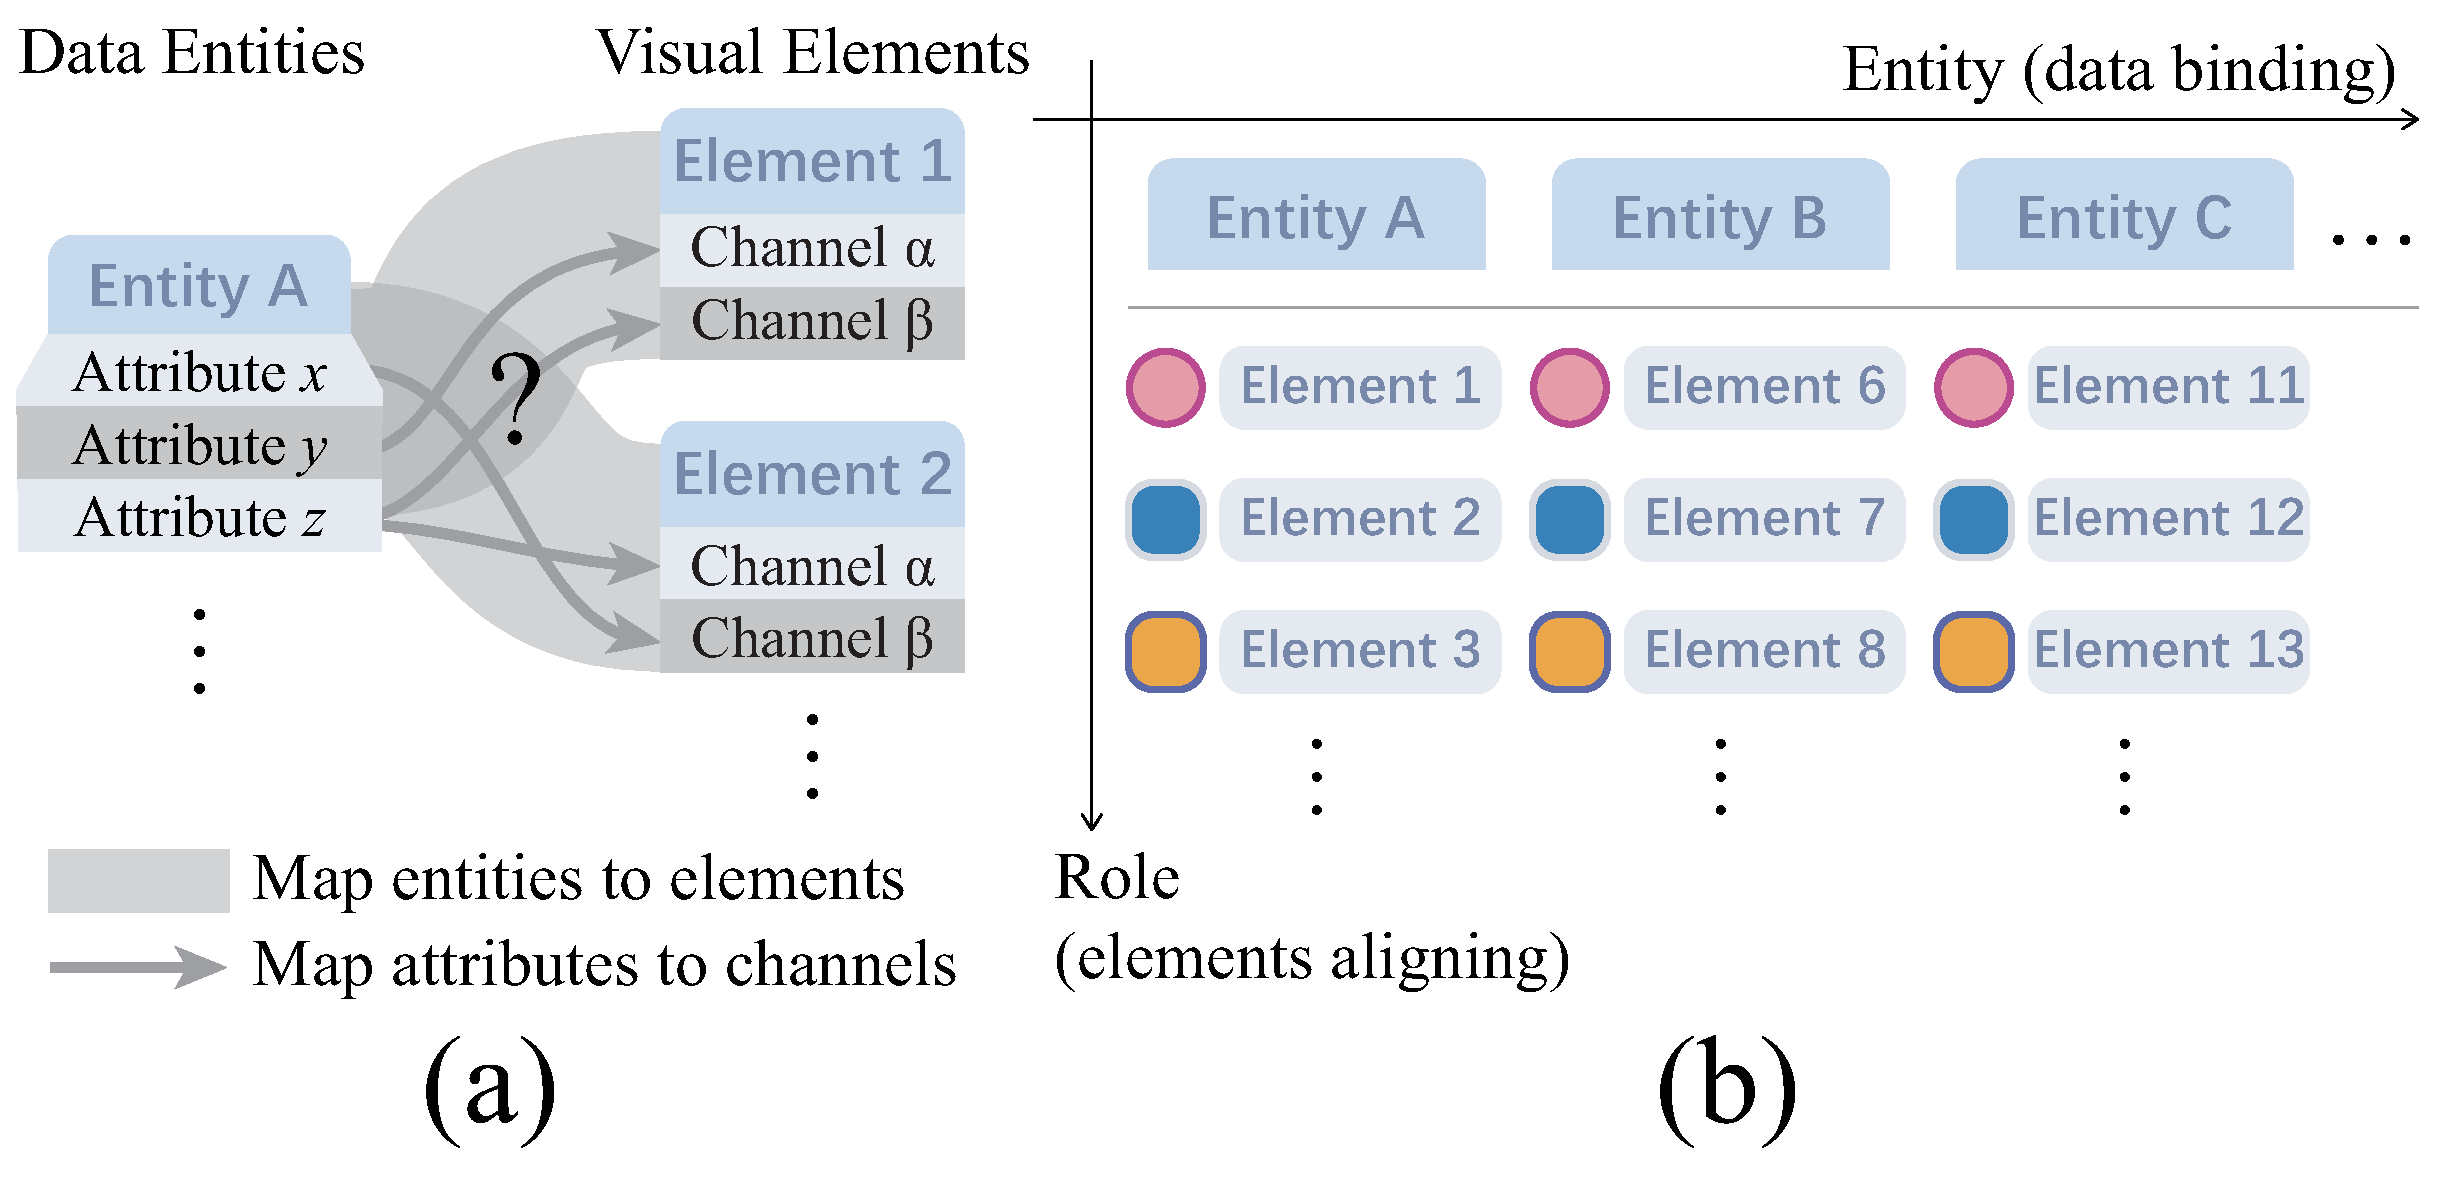
\includegraphics[width=1\columnwidth]{figures/ElementAligning.eps}
    \caption{(a) The target of our visual encoding detection technique; and (b) effect of the data-binding step and the elements-aligning step.}
    \label{fig:ElementAligning}
\end{figure}

% xxxx 等人的工作为我们提供了一个良好的思路,但他们的工作存在一些限制
A tool proposed by Harper and Agrawala~\cite{DBLP:conf/uist/HarperA14} provides a creative perspective for visual encoding extraction.
Although that tool can be extended to support simple node-link diagrams (where each data entity is encoded as only one element), several limitations exist:
\begin{compactenum}
% 1. 其需要创作者使用d3的数据绑定,才能发挥__data__的作用;使用其他工具,或者未将数据绑定到元素上时则无法使用该方法;
\item The D3's data-binding feature is required within the tool so by the ``\texttt{\_\_data\_\_}'' attribute of visual elements can be acquired. 
It cannot deal with general SVG-format visualizations without data bound to visual elements.

% 2. 其只能检验属性和视觉通道之间是否存在线性映射或者类别性映射。
\item It only supports the linear mapping and the categorical mapping and cannot maintain situations with complex visual mappings.
\end{compactenum}
These obstacles prevent it from extracting visual encodings from node-link diagrams created in the general SVG format.

% 我们针对节点链接图的场景,提出了一个数据绑定的策略,通过不断调整输入的数据,检查输出的变化,从而获取数据到svg元素之间的映射关系以及属性到视觉通道之间的映射方式,以解决以上两个问题。
For node-link diagrams, we introduce a new technique to solve such limitations.
Our technique incorporates the source code and the underlying graph data.
The key idea is regarding the source code as a black box.
Our technique modifies the input graph data and detects changes in the output SVG to obtain mappings between data entities and visual elements.
It overcomes the limitations by three steps (Figure~\ref{fig:VisualEncodings}):
(1) \textbf{Data binding} binds elements to different data entities.
(2) \textbf{Elements aligning} aligns elements according to their \textit{roles}. 
(3) \textbf{Encoding mapping} detects correlations among attributes, elements, and visual channels.

\subsubsection{Data Binding} \label{sec:databinding}
To detect mappings between \textbf{\textit{data entities}} and \textbf{\textit{visual elements}}, 
we modify attribute values of data entities and record corresponding visual element changes so as to construct mappings between the modified entity and the changed elements.
However, directly modifying attributes may deform the attribute distribution, and this can influence visual mappings so that elements related to other data entities may also be changed.
% 节点的size属性线性映射到编码该节点的圆形的半径r上,r[i] = (size[i] - min(size)) / (max(size) - min(size)) * max_radius
For example, the node's \texttt{size} attribute is linearly mapped into the radius of the \texttt{<circle>} element encoding the node: 
% $$radius_i = \frac{size_i - min(size)}{max(size) - min(size)} * radius_{max}$$
$radius_i = (size_i - min(size)) / (max(size) - min(size)) * radius_{max}$.
Modifying $size_i$ may broaden the attribute range and changes the linear mapping defined by the attribute range.
We prevent this by merely swapping attributes of two entities rather than modifying them, so that no new data is introduced and the distribution is preserved.
We take nodes as an example.
After swapping all two nodes' attributes, visual elements that differ from the previous are regarded as two nodes' corresponding elements.
For example, after swapping nodes B and C in Figure~\ref{fig:DataBinding} (b), elements 1 to 4 are changed.
All these changed elements correspond to nodes B and C because only B and C are swapped.
After swapping the node B with the node A in Figure~\ref{fig:DataBinding} (c), elements 2 and 3 are changed twice (Figure~\ref{fig:DataBinding} (b) and (c)), thus they correspond to node B because only node B are swapped twice.
% To ensure all elements of node B are detected, we swap it with all the other nodes.
Each node will be swapped with all other nodes to ensure that all elements belonging to it are detected.
After swapping all nodes, the entire node-to-element mapping is constructed (Figure~\ref{fig:DataBinding} (d)).
Node entities are bound to their corresponding elements.
The link-to-element mapping is constructed in the same way.
Because swapping two nodes may influence their related links, node-related elements can contain elements corresponding to links.
We remove elements corresponding to links from the node-to-element mappings.
Two parts ($entity$ and $element$) of the mapping relationship are solved.

\begin{figure}
    \centering
    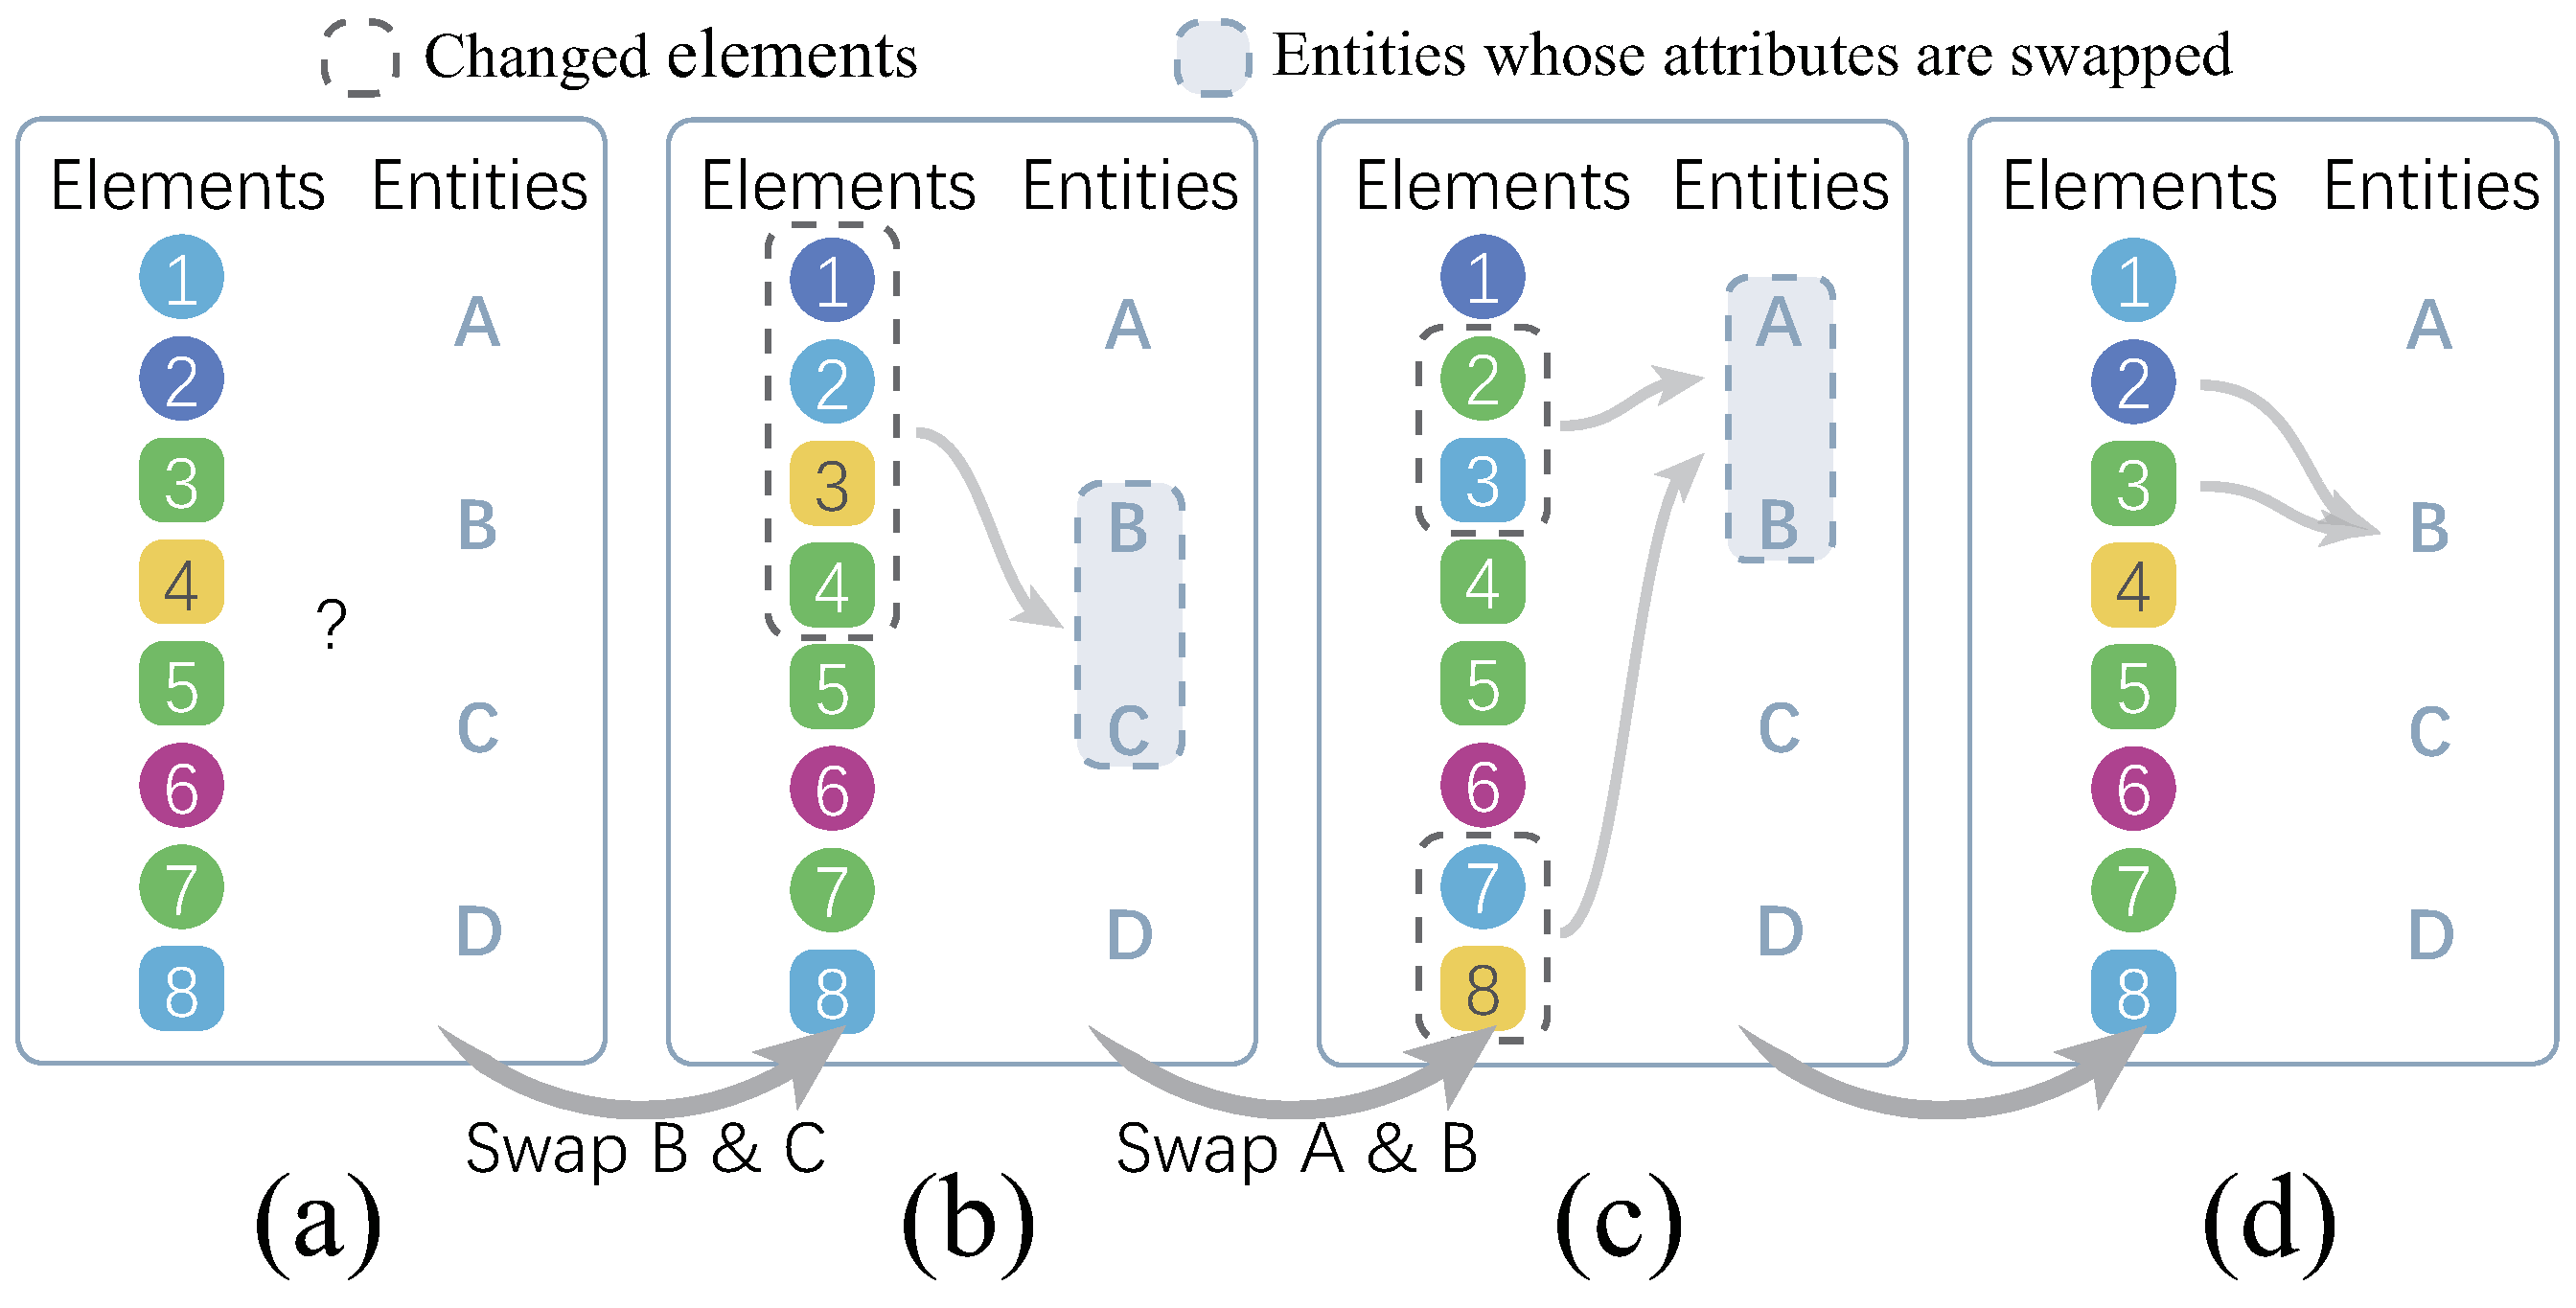
\includegraphics[width=1\columnwidth]{figures/DataBinding.eps}
    \caption{Data binding is achieved by swapping attributes of data entities. (a) Visual mappings between original visual elements and data entities are unknown. (b) After swapping attributes of entities B and C, the appearance of elements 1 to 4 is changed. Thus, entities B and C correspond to elements 1 to 4. (c) After swapping attributes of entities A and B, the appearance of elements 2, 3, 7, and 8 is changed. Thus, entities A and B correspond to these elements. (d) After swapping B with A and C, elements 2 and 3 change twice. We can map entity B to elements 2 and 3.}
    \label{fig:DataBinding}
\end{figure}

\subsubsection{Elements Aligning}
The data-binding step only binds visual elements into different data entities (the horizontal direction in Figure~\ref{fig:ElementAligning} (b)).
The roles of different elements are unknown.
The \textit{role} of an element is defined as a function that maps attributes to visual channels:
\begin{equation}
    role :=  \{attribute: value\} \mapsto \{channel: appearance\}
\end{equation}
% 两个元素相同角色,当且仅当,在它们所对应的数据实体的所有属性都相同时,它们的channels也都一样。
Two elements have the same role iff given arbitrary same inputs (all attributes of their corresponding entities), their outputs (all their visual channels) are the same.
For the example in Figure~\ref{fig:VisualEncodings}, 
roles of all three left inner rectangles are the same,
because if we swap all attributes of nodes A and B, node A's left rectangle before swapping will be same to node B's left rectangle after swapping regarding all their visual channels such as \texttt{x}, \texttt{y}, \texttt{fill}, and \texttt{height}.
They are aligned to classify their roles (the vertical direction in Figure~\ref{fig:ElementAligning} (b)).
% The \textit{role} can be regarded as a function that takes data attributes as input and assign values for visual element channels.
% Elements across different data entities are regarded as the same role if their effects are the same.
% Elements within the same role should appear exactly the same when their own nodes have exactly same attributes.
% 通过测试两个元素在同一属性输入时是否表现一致,来判断它们是否属于一种角色。
Different elements' role identity can be determined by swapping their corresponding data entities along with the data binding step, because all attributes of one entity before swapping are the same to the counterpart of the other one after swapping.
For example, in Figure~\ref{fig:DataBinding} (b), after swapping entity B with entity C, element 1 appear same to element 2 before swapping in Figure~\ref{fig:DataBinding} (a). Thus, elements 1 and 2 can be aligned into the same role.
We clarify the binding among visual elements, data attributes, and visual channels, which is conducive to the subsequent steps.
% 这样做的意义:能够使得数据和可视化之间的绑定更加清晰,有利于后续步骤的进行。


\subsubsection{Encoding mapping}\label{sec:encodingmapping}
The previous two steps classify elements according to two dimensions (the entity and the role) to solve \textbf{Q\ref{qstn:composition}}.
% 到此为止,我们已经已经知道每个实体是由哪些不同角色的元素组成,足够回答第一个问题
However, correlations between visual channels and data attributes are not determined.
% 我们继续以节点为例。
We continue to take nodes as an example.
% 为了检验一个属性究竟被编码在了哪些视觉通道上,我们通过shuffle所有节点的某个属性,观察视觉通道发生的变化。
We detect related visual channels of an attribute by shuffling all nodes' attributes and observing visual channel changes of their corresponding elements.
% 变化可以被定义为,某个属性引起某些元素的某些视觉通道的变化。
One correlation is defined as ``which \textit{attribute} changes which \textit{visual channel} of which \textit{element}''. We formalize it as:
\begin{equation}
    correlation := ( attribute, element, channel )
\end{equation}
% 然后我们根据不同的element角色,对这些发生的变化进行合并。
We merge different correlations according to the role of elements.
Thus, we replace the $element$ in the correlation's definition with $role$.
We obtain the entire correlation set of different roles to solve \textbf{Q\ref{qstn:encodings}}.
% It generates more comprehensive mappings between attributes and visual channels for elements of different roles.

Moreover, we identify the category of correlations to solve \textbf{Q\ref{qstn:correlation}}.
It requires the classification of attribute types and channel types.
We support numerical attributes and categorical attributes in \ApproachName.
List attributes and dictionary attributes are separated into multiple numerical attributes or categorical attributes (e.g.,\texttt{[1, 2, 3]}, \texttt{\{"year":2021,"month":03\}}).
We regard all visual channels as numerical (colors can be divided into RGB channels which are numerical).
However, numerical data can be used as categorical data if there are only a few classes of values.
For example, natural numbers are often used as categorical attributes such as labels, groups, and classes.
Thus, for numerical data, we must compare the number of unique values and their entries to determine whether it is numerical or categorical.
We set up a parameter $\alpha$ to make the distinction: if all values of the attribute are natural numbers and
the number of an attribute's unique values is less than $\alpha$ percent of the number of data entities, we regard the attribute as categorical.
% 我们根据属性和通道的类型来定义关系的类型
We identify the type of correlation by the type of attribute and channel:
\begin{compactitem}
    \item \textbf{The channel and attribute are categorical} or \textbf{the channel is categorical while the attribute is numerical}. 
    % 为了描述不同的channel取值所代表的的含义。我们为每类不同的channel记录了它们所对应的属性的取值范围。
    In order to describe the meanings of different channel values,
    We record the value range of the attribute for each category of channel values.
    % 假如在这种关系下,不同类别的channel对应的属性取值有交叉,我们则会抛弃这种关系,因为它具有歧义。
    If the attribute values corresponding to different channel values intersect, we discard this correlation because it is ambiguous.
    
    \item \textbf{The channel and attribute are numerical}. We compute the Pearson's Correlation Coefficient and test whether the correlation is positive, negative, or uncorrelated with the coefficient and the significance test's p-value. We take the attribute as a factor that influences the visual channel when the absolute value of the coefficient is larger than $\theta$, and the $p$-value of the significance test is less than $\alpha$. We set $\theta = 0.5$ and $\alpha = 0.05$ by default, both parameters can be adjusted on-demand.
\end{compactitem}
The correlation type where \textbf{the channel is numerical while the attribute is categorical} is not supported because it is counterintuitive.


\begin{algorithm}[!t]
    \renewcommand\arraystretch{1.2}
    \caption{ Visual Encodings Textualization }
    \label{alg:textualize}
    \begin{algorithmic}[1]
        % \Require
            % $G=(V=\{v_1, v_2, ..., v_n\}, E=\{e_1, e_2, ..., e_n\})$: a graph;
        % \Ensure
            % $C$: the potential condition set
        % \State Init conditions $C=\varnothing$, false conditions $FC=\varnothing$
        \State // Describing Nodes
        \State Describing \textbf{Q\ref{qstn:composition}}: what \textit{elements} (\textit{roles}) does a node consist of? \label{alg:VsEnNodeConsist}
        \For {each \textit{role} in a node} \label{alg:VsEnEachRole}
            \If {its \texttt{tagName} does not encode any \textit{attribute}}
                \For {each \textit{visual channel} that encodes some attributes}
                    \State Describing \textbf{Q\ref{qstn:encodings}}: how \textit{channel} encodes \textit{attributes}? \label{alg:VsEnQ2-1}
                    \State Describing \textbf{Q\ref{qstn:correlation}}: the type of their \textit{correlations}
                    \label{alg:VsEnQ3-1}
                \EndFor
            \EndIf
            \If {its shape (\texttt{tagName}) encodes some attributes}
                \For {each \textit{visual channel} that all shapes share}
                    \State // e.g., \texttt{fill} and \texttt{stroke-width}
                    \State Describing \textbf{Q\ref{qstn:encodings}}: how \textit{channel} encodes \textit{attributes}? \label{alg:VsEnQ2-2}
                    \State Describing \textbf{Q\ref{qstn:correlation}}: the type of their \textit{correlations}
                    \label{alg:VsEnQ3-2}
                \EndFor
                \State Describing all its shapes \label{alg:VsEnTagName}
                \For {each shape (\texttt{tagName})}
                    \State Describing \textbf{Q\ref{qstn:encodings}}: how \textit{channel} encodes \texttt{tagName}? \label{alg:VsEnQ2-3}
                    \State Describing \textbf{Q\ref{qstn:correlation}}: the type of their \textit{correlations}
                    \label{alg:VsEnQ3-3}
                    \For {each \textit{visual channel} that this shape holds}
                        \State // e.g., \texttt{rx} and \texttt{ry}
                        \State Describing \textbf{Q\ref{qstn:encodings}}: how \textit{channel} encodes \textit{attributes}? \label{alg:VsEnQ2-4}
                        \State Describing \textbf{Q\ref{qstn:correlation}}: the type of their \textit{correlations} \label{alg:VsEnQ3-4}
                    \EndFor
                \EndFor
            \EndIf
        \EndFor
        \State // Describing Links ...
    \end{algorithmic}
\end{algorithm}

\subsubsection {Template-based Textualization}
Descriptions of visual encodings are generated based on several templates.
There are logical and hierarchical relationships in the narration of these visual encodings.
Algorithm~\ref{alg:textualize} summarizes the overall logic for describing visual encodings.
We describe nodes and links respectively.
Elements of different roles composing a node are narrated separately, for example,
\textit{``Each @node consists of @4 different elements.''} (line~\ref{alg:VsEnNodeConsist}),
\textit{``The @first element is a @\texttt{<rect>}.''} (line~\ref{alg:VsEnEachRole}).
% 为了标记模板中用于填充信息的部分,我们对这些位置进行了高亮。
To mark the placeholders of templates that are used to fill in the information, we place a @ sign before the words that fill into these placeholders.
For visual channels that encode attributes, we describe their correlation to solve \textbf{Q\ref{qstn:encodings}} and \textbf{Q\ref{qstn:correlation}}.
For example, \textit{``Its @fill encodes the attribute @group.''} (line~\ref{alg:VsEnQ2-1}).
% , \textit{``The greater the attribute @value is, the @greater its @stroke-width is.''} (line~\ref{alg:VsEnQ3-1},~\ref{alg:VsEnQ3-2},~\ref{alg:VsEnQ3-3}, and~\ref{alg:VsEnQ3-4}).
If the correlation is categorical-to-categorical, we describe different categories separately: \textit{``When the value of @group is @2, its @fill is changed into @darkorange (\#ff7f0e).''} (Colors are described as the most similar color in a predefined set of colors with 146 different names).
If the correlation is numerical-to-numerical, we describe whether the value of the channel will increase or decrease with the growth of the attribute's value: \textit{``The greater the attribute @value is, the @greater its @stroke-width is.''} (line~\ref{alg:VsEnQ3-1}).

If the shape is used to encode some attributes, the logic of description is different.
We first describe common channels shared by different shapes (lines~\ref{alg:VsEnQ2-2} and~\ref{alg:VsEnQ3-2}) and then narrate different shapes:
\textit{``Its tagName varies from @\texttt{<circle>} and @\texttt{<rect>}.''} (line~\ref{alg:VsEnTagName}), \textit{``When the value of @country is @France, its tagName is changed into @\texttt{<circle>}``} (lines~\ref{alg:VsEnQ2-3} and~\ref{alg:VsEnQ3-3}), and \textit{``Its @radius encodes the attribute @votes. The greater the @votes, the @greater its @radius.''}(lines~\ref{alg:VsEnQ2-4} and~\ref{alg:VsEnQ3-4}).

\subsection{Interpreting Layout Intention}
% Layouts of attributed graphs have been categorized into attribute-based layouts~\cite{} and topology-based layouts~\cite{} by Nobre et al.~\cite{DBLP:journals/cgf/NobreMSL19}.
Nobre et al.~\cite{DBLP:journals/cgf/NobreMSL19} categorized layouts of attributed graphs into attribute-based layouts~\cite{DBLP:journals/tvcg/ElzenW14, DBLP:journals/tvcg/Guo09} and topology-based layouts~\cite{DBLP:journals/spe/FruchtermanR91, DBLP:journals/cgf/KruigerRMKKT17, DBLP:journals/tvcg/GansnerHN13, DBLP:journals/tvcg/ZhuCHHLZ21}.
The core of describing layout intention is to determine whether the layout is attribute-based or topology-based, is handled in two steps: 

\textbf{1) Capturing the position of each node}.
To capture each node's position, we compute a bounding box for elements detected in Section~\ref{sec:databinding}.
The bounding box of a node is the smallest rectangle that contains all its corresponding elements.
We take the centroid of the bounding box as the position of the node.

\textbf{2) Determining the layout type.} 
The attribute-based category of layouts is defined as algorithms that mapping node attributes to the two dimensions ($x$ and $y$) of the Cartesian coordinate. 
We utilize the Pearson correlation test same to Section~\ref{sec:encodingmapping} to test whether an attribute relates to the layout.
% For each attribute of the node, we test whether it relates to the layout.
% The test is similar to the correlation test in Section~\ref{sec:encodingmapping}.
% If the test does not suggest any attribute as the impact factor, we begin to test whether it is topology-based.
For topology-based layouts, we assume that their graph geodesic distance influences the Euclidean distance between two nodes.
The Pearson correlation coefficient can also be used to test the correlation.
We assume that with the conditions that the Pearson correlation coefficient is more significant than $\theta$ and $p$-value is smaller to $\alpha$, the layout is topology-based.

Thus we first perform a pre-study to validate our hypothesis.
% 找N个不同的数据集(跨不同领域),找几种不同种类的拓扑based的layout;检验他们的pearson值,p值等等;比较它们在随机布局下的结果;
We prepare 15 different graph datasets from~\cite{DBLP:journals/tvcg/ZhuCHHLZ21}.
The number of their nodes varies from 72 to 1083, and the number of their links varies from 75 to 8677.
They are collected from diverse areas such as literature, music, research, and social media.
We layout them using five different kinds of topology-based layouts with default parameters: FM$^3$~\cite{hachul2004drawing}, Fruchterman-Reingold spring layout (F.R.)~\cite{DBLP:journals/spe/FruchtermanR91}, Stress Majorization (S.M.)~\cite{DBLP:conf/gd/GansnerKN04}, Pivot MDS (PMDS)~\cite{DBLP:conf/gd/BrandesP06}, and Radial Tree layout (R.T.)~\cite{DBLP:conf/infovis/Jankun-KellyM03}.
% 我们还检验了随机布局是否也符合我们的假设
We also test whether the random layout conforms to our assumption.
We highlight cells where the Pearson correlation coefficient is smaller than $\theta$ in Table~\ref{tab:pearson-correlation}.
They suggest that correlations between the euclidean distance and the graph geodesic distance are weak.
$p$-values are all zero for the five topology-based layouts in all 15 datasets.
They suggest strong correlations between the Euclidean distance and the graph geodesic distance.
However, nine of 15 datasets with the random layout also produce $p$-values less than $\alpha$, which suggests they are significant.

% 这些基于拓扑的布局产生的节点位置,能够使节点间的欧式距离反应它们的拓扑距离。
Two tables indicate that in most cases, the Euclidean distance between two nodes reflects their graph geodesic distance with topology-based layouts.
% 在大部分情况下,使用pearson 相关系数>0.6且p-value<0.05来检验是否该布局为拓扑布局是可行的。
Thus, it is feasible to study whether the layout is a topological layout with the first condition established (the Pearson correlation coefficient$>\theta$).

Descriptions of the layout intention are also template-based.
For attribute-based layout, we narrate that: \textit{``The @x-coordinate encodes the attributes @votes''}.
The description for topology-based layouts is: \textit{``The layout is a topology-based layout, which means the farther the topology distance between two nodes, the farther the distance between them''}.
When the layout does not conform to the two categories, it yields: \textit{``The layout is neither an attribute-based layout nor a topology-based layout.''}.

\begin{table}[ht]
\caption{\label{tab:pearson-correlation}The Pearson correlation coefficients testing correlations between Euclidean distances and graph geodesic distance with 15 graphs and 6 different layouts. Cells with coefficients less than $\theta=0.5$ are highlighted.}

\setlength{\tabcolsep}{1.5mm}{

% \resizebox{\textwidth}{15mm}{
\begin{tabular}{lllllll}
\hline
Dataset       & FM$^3$ & F.R.           & S.M.  & PMDS  & R.T.           & Random          \\ \hline
dwt\_72       & 0.894                 & 0.552          & 0.94  & 0.897 & 0.714          & \textbf{-0.003} \\
lesmis        & 0.804                 & 0.728          & 0.815 & 0.779 & 0.504 & \textbf{-0.03}  \\
bcsstk09      & 0.967                 & 0.610          & 0.971 & 0.947 & 0.754          & \textbf{-0.008} \\
cage8         & 0.658                 & 0.678          & 0.725 & 0.701 & \textbf{0.307} & \textbf{-0.002} \\
can\_96       & 0.835                 & 0.824          & 0.855 & 0.869 & \textbf{0.426} & \textbf{0.013}  \\
dwt\_1005     & 0.969                 & 0.561          & 0.974 & 0.972 & 0.623          & \textbf{0.007}  \\
dwt\_419      & 0.979                 & \textbf{0.391} & 0.987 & 0.987 & 0.775          & \textbf{-0.004} \\
grid17        & 0.968                 & 0.551          & 0.976 & 0.964 & 0.738          & \textbf{-0.007} \\
jazz          & 0.826                 & 0.821          & 0.813 & 0.786 & \textbf{0.297} & \textbf{0.004}  \\
mesh3e1       & 0.99                  & 0.502          & 0.996 & 0.995 & \textbf{0.465} & \textbf{0.002}  \\
netscience    & 0.901                 & 0.573          & 0.93  & 0.919 & 0.752          & \textbf{-0.018} \\
price\_1000   & 0.783                 & \textbf{0.376} & 0.808 & 0.786 & 0.727          & \textbf{-0.007} \\
rajat11       & 0.753                 & 0.670          & 0.868 & 0.847 & 0.618          & \textbf{-0.064} \\
soc-wiki-Vote & 0.798                 & 0.775          & 0.821 & 0.757 & \textbf{0.316} & \textbf{-0.01}  \\
visbrazil     & 0.937                 & 0.828          & 0.941 & 0.958 & 0.758          & \textbf{0.01}   \\ \hline
\end{tabular}}
\end{table}

% \begin{table}[ht]
% \caption{\label{tab:pearson-pvalue}Pearson p-value(TODO).}

% \setlength{\tabcolsep}{1.9mm}{

% \begin{tabular}{lllllll}
% \hline
% Dataset       & FM$^3$ & F.R. & S.M. & PMDS & R.T. & Random         \\ \hline
% dwt\_72       & 0                     & 0    & 0    & 0    & 0    & \textbf{0.842} \\
% lesmis        & 0                     & 0    & 0    & 0    & 0    & 0.021          \\
% bcsstk09      & 0                     & 0    & 0    & 0    & 0    & 0              \\
% cage8         & 0                     & 0    & 0    & 0    & 0    & 0.027          \\
% can\_96       & 0                     & 0    & 0    & 0    & 0    & \textbf{0.203} \\
% dwt\_1005     & 0                     & 0    & 0    & 0    & 0    & 0              \\
% dwt\_419      & 0                     & 0    & 0    & 0    & 0    & \textbf{0.111} \\
% grid17        & 0                     & 0    & 0    & 0    & 0    & \textbf{0.060} \\
% jazz          & 0                     & 0    & 0    & 0    & 0    & \textbf{0.421} \\
% mesh3e1       & 0                     & 0    & 0    & 0    & 0    & \textbf{0.604} \\
% netscience    & 0                     & 0    & 0    & 0    & 0    & 0              \\
% price\_1000   & 0                     & 0    & 0    & 0    & 0    & 0              \\
% rajat11       & 0                     & 0    & 0    & 0    & 0    & 0              \\
% soc-wiki-Vote & 0                     & 0    & 0    & 0    & 0    & 0              \\
% visbrazil     & 0                     & 0    & 0    & 0    & 0    & 0.025          \\ \hline
% \end{tabular}}

% \end{table}

\subsection{Interactive Descriptions}
Descriptions can be enhanced by interactions because they are generated with corresponding elements.
For example, descriptions about nodes correspond to nodes related elements.
When audiences hover on one sentence of description, we highlight related elements to help the user capture the description's target.
We develop an interactive web-based interface by JavaScript to support generating interactive descriptions (Figure~\ref{fig:interface}) with \ApproachName.
Creators can write visualization code in the Code Editor and input the graph data in the Data Editor.
\ApproachName~generates the visualization results and their corresponding interactive descriptions.


\begin{figure}[ht]
    \centering
    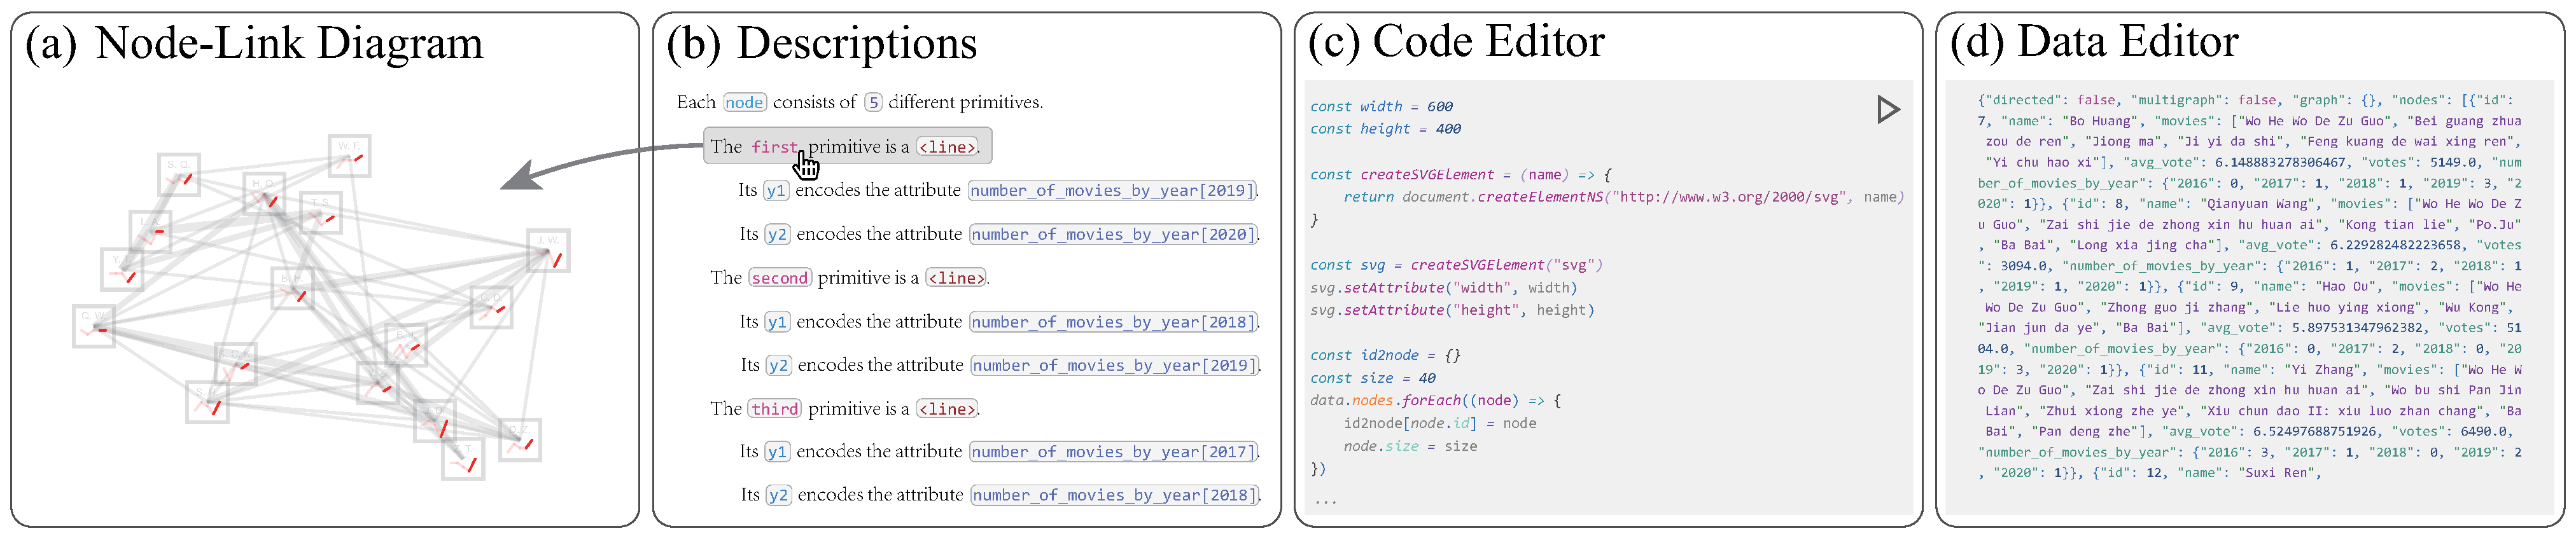
\includegraphics[width=1\columnwidth]{figures/interface.eps}
    \caption{The interface consists of four parts: (a) the node-link diagram view, (b) the descriptions view that shows the descriptions generated by \ApproachName, (c) the code editor view where creators can edit their visualization creation code, and (d) the data editor where creators input the graph data.}
    \label{fig:interface}
\end{figure}